\subsection{LED Blink Project}

This project focuses on the interaction with a microcontroller's hardware, specifically controlling a LED. The goal is to make a LED blink every 1000 milliseconds. To achieve this, we use the HAL (Hardware Abstraction Layer) library provided by STM.

\subsubsection{Hardware Abstraction Layer}

The HAL library is an Application Programming Interface (API) that abstracts the details of the microcontroller's hardware. This means that we can write code that interacts with the hardware in a high-level and portable way.

The HAL library provides a function, \texttt{HAL\_GPIO\_TogglePin}, that allows us to alter the state of a pin. This function takes two arguments: the GPIO port and the pin number. For the LED, the GPIO port is \texttt{GPIOA} (0x40000000) and the pin number is 5 (0x20 is the bitmask):

\subsubsection{Pin Control}

To control the LED on a NUCLEO-F103RB board, the HAL library needs to write some bits in memory. From the documentation of the board, the GPIO Register Map has the structure showed in the figure \ref{fig:gpio_register_map}.

\begin{figure}[ht]
    \centering
    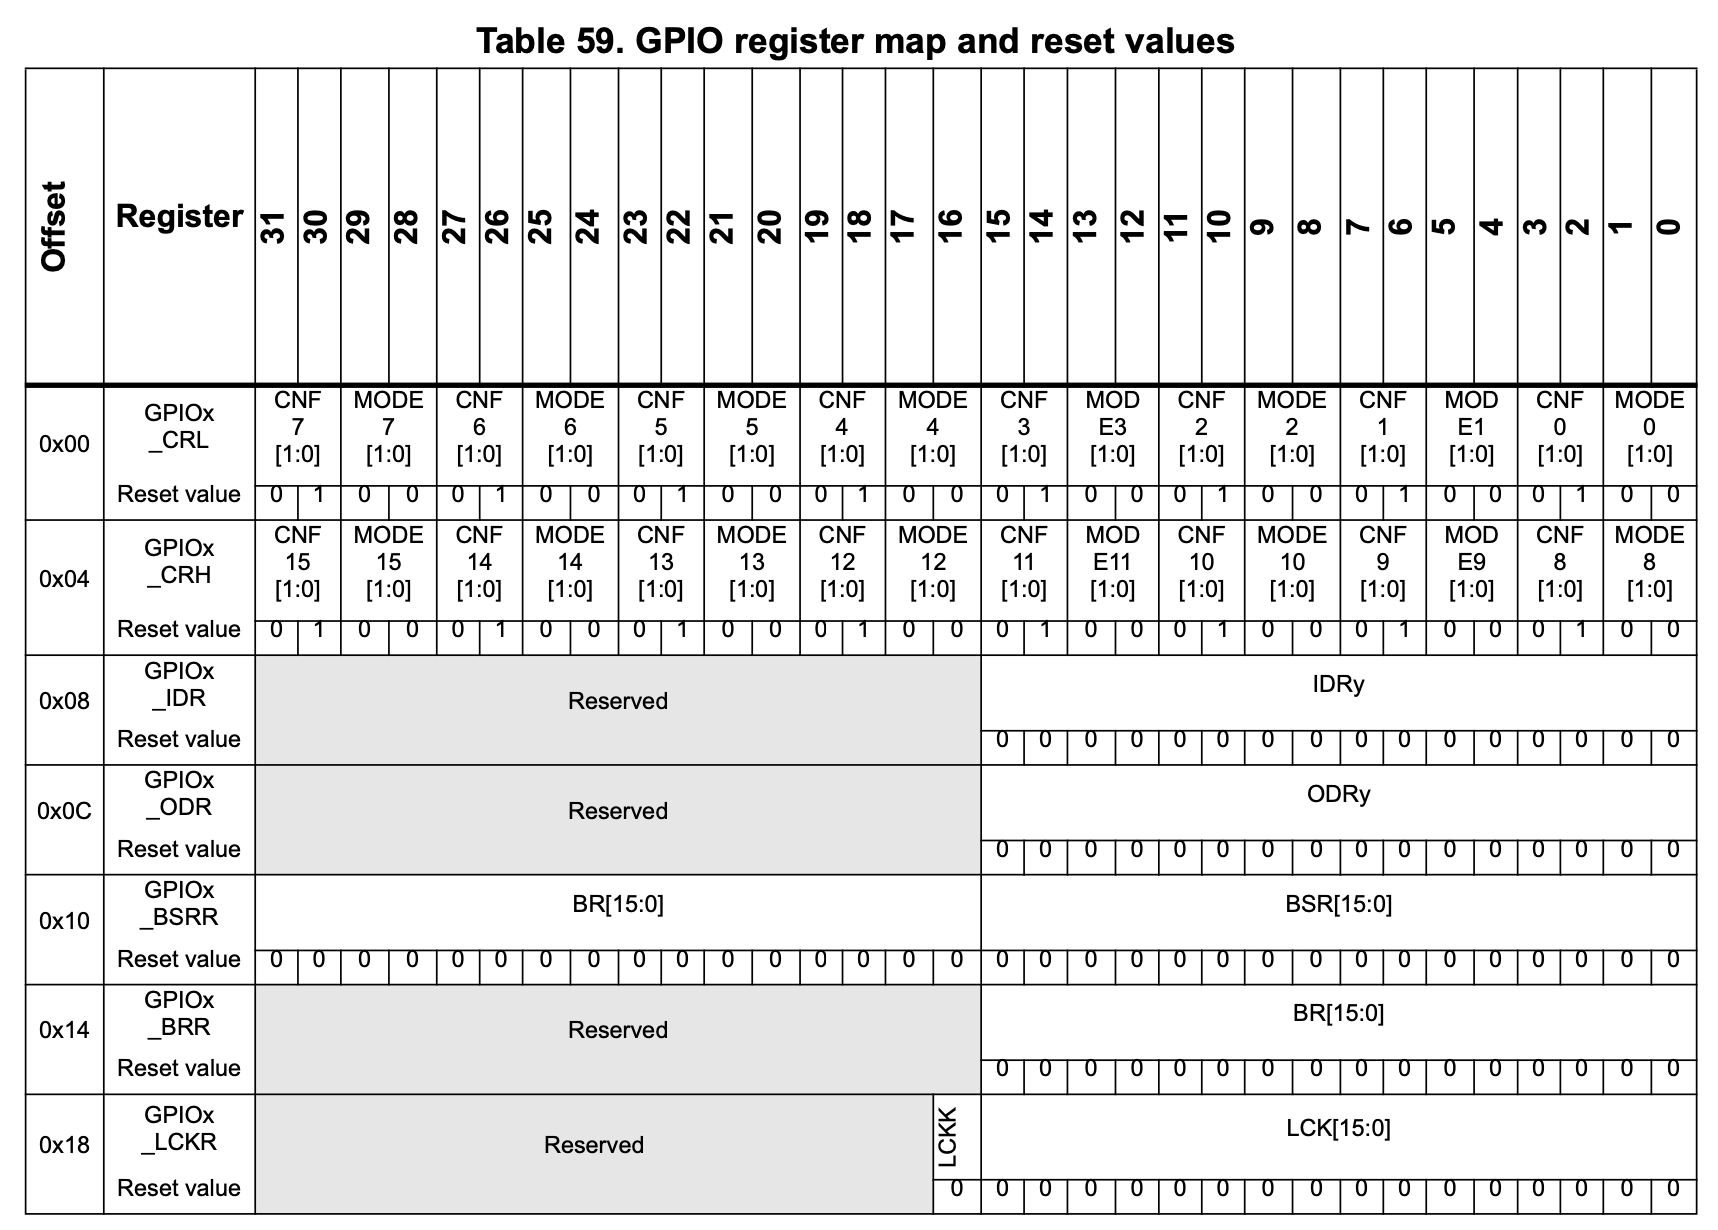
\includegraphics[width=0.8\textwidth]{images/projects/gpio_register_map.png}
    \caption{GPIO Register Map}
    \label{fig:gpio_register_map}
\end{figure}

To set or reset a pin, the BSSR (Bit Set/Reset Register) is used. The first 16 bits of the BSSR register are used to set, while the last 16 bits are used to reset.

To toggle a pin, first the current value is taken from the ODR (Output Data Register) and then the BSSR low register is written with the inverse of the current value, while the BSSR high register is written with the current value.